\documentclass[aspectratio=169]{beamer}

\usetheme{Boadilla}
\setbeamertemplate{navigation symbols}{}

\usepackage[T1]{fontenc}
\usepackage[utf8]{inputenc}
\usepackage{booktabs}
\usepackage{array}
\usepackage{multirow}
\usepackage{amsmath}
\usepackage{graphicx}
\usepackage{xcolor}

% ── Custom color palette ─────────────────────────────────────────────────────
\definecolor{qNavy}{RGB}{15, 40, 90}
\definecolor{qMid}{RGB}{0, 100, 180}
\definecolor{qLight}{RGB}{220, 232, 245}
\definecolor{qGold}{RGB}{200, 160, 40}

\setbeamercolor{frametitle}{bg=qNavy, fg=white}
\setbeamercolor{frametitle right}{bg=qNavy}
\setbeamercolor{title}{fg=white}
\setbeamercolor{subtitle}{fg=qLight}
\setbeamercolor{author}{fg=qLight}
\setbeamercolor{date}{fg=qLight}
\setbeamercolor{palette primary}{bg=qNavy, fg=white}
\setbeamercolor{palette secondary}{bg=qMid, fg=white}
\setbeamercolor{palette tertiary}{bg=qNavy!70, fg=white}
\setbeamercolor{palette quaternary}{bg=qNavy, fg=white}
\setbeamercolor{itemize item}{fg=qMid}
\setbeamercolor{itemize subitem}{fg=qMid!70}
\setbeamercolor{enumerate item}{fg=qMid}
\setbeamercolor{block title}{bg=qNavy, fg=white}
\setbeamercolor{block body}{bg=qLight, fg=black}
\setbeamercolor{structure}{fg=qMid}
\setbeamercolor{background canvas}{bg=white}

\setbeamertemplate{title page}{%
  \begin{tikzpicture}[remember picture, overlay]
    \fill[qNavy] (current page.north west) rectangle (current page.south east);
  \end{tikzpicture}%
  \vspace{2em}
  \begin{center}
    {\Large\color{white}\textbf{\inserttitle}}\\[0.5em]
    {\small\color{qLight}\insertsubtitle}\\[1.5em]
    {\color{qLight}\insertauthor}\\[0.3em]
    {\color{qLight}\insertdate}
  \end{center}
}

\usepackage{tikz}

\title{Strategy-Space Modeling for Interpretable Quant Research}
\subtitle{From Linear Combination to ML-Guided Allocation on GLD (SPDR Gold Shares ETF)}
\author{Joon Chun}
\date{April 2026}

\begin{document}

% ── Slide 1: Title ───────────────────────────────────────────────────────────
\begin{frame}
  \titlepage
\end{frame}

% ── Slide 2: Outline ─────────────────────────────────────────────────────────
\begin{frame}{Outline}
  \begin{enumerate}
    \item \textbf{Motivation} \hfill \small\textit{slides 3--4}\\[-0.1em]
      \footnotesize From polynomial basis functions to strategy-space modeling
    \normalsize\vspace{0.3em}

    \item \textbf{Four Strategy Families} \hfill \small\textit{slides 5--10}\\[-0.1em]
      \footnotesize Adaptive Band, MA Crossover, Adaptive Vol.\ Band, Fear-Greed
    \normalsize\vspace{0.3em}

    \item \textbf{Stage A: Single Strategy} \hfill \small\textit{slide 11}\\[-0.1em]
      \footnotesize Each strategy alone captures only a fraction of the market
    \normalsize\vspace{0.3em}

    \item \textbf{Stage B: Ensemble} \hfill \small\textit{slides 12--15}\\[-0.1em]
      \footnotesize Combining signals via constrained optimization
    \normalsize\vspace{0.3em}

    \item \textbf{Stage C: ML-Guided} \hfill \small\textit{slides 16--20}\\[-0.1em]
      \footnotesize 40-column design matrix, supervised learning, continuous exposure
    \normalsize\vspace{0.3em}

    \item \textbf{Results \& Analysis} \hfill \small\textit{slides 21--24}\\[-0.1em]
      \footnotesize Three-stage comparison, update frequency, hold horizon
    \normalsize\vspace{0.3em}

    \item \textbf{Live Signal Example} \hfill \small\textit{slide 25}\\[-0.1em]
      \footnotesize Stage C running in production on Raspberry Pi
    \normalsize\vspace{0.3em}

    \item \textbf{Next Steps \& Conclusion} \hfill \small\textit{slides 26--27}
  \end{enumerate}
\end{frame}

% ── Slide 3: Starting Point ──────────────────────────────────────────────────
\begin{frame}{Starting Point}
  \begin{itemize}
    \item \textbf{Asset}: GLD — SPDR Gold Shares ETF, a liquid gold commodity fund traded on NYSE.
          Daily price data from 2019--2024.
    \item The project started from a mathematical question, not a trading rule.
    \item In class, we studied model selection using polynomial basis functions:
    \[
      1,\ x,\ x^2,\ \dots,\ x^d
    \]
    \item That raised the main idea:
    \[
      \text{Can trading strategies also be treated as basis functions?}
    \]
    \item If a strategy maps a market state into a numerical score,
          it can be evaluated across dates and placed into a design matrix.
  \end{itemize}
\end{frame}

% ── Slide 3: Function Space Analogy ─────────────────────────────────────────
\begin{frame}{Function Space Analogy}
  \small
  \begin{tabular}{lll}
    \toprule
    Concept & Polynomial Model & Strategy Model \\
    \midrule
    basis function  & \(1, x, x^2, \dots\)   & strategy signal functions \\
    data point      & \(x_i\)                 & market state at date \(t_i\) \\
    matrix entry    & \(\phi_j(x_i)\)         & strategy score \(s_j(t_i)\) \\
    model selection & choose degree / penalty & choose strategy / penalty \\
    target          & observed \(y_i\)        & future cumulative return \\
    \bottomrule
  \end{tabular}

  \vspace{0.6em}
  Core design matrix:
  \[
    A_{ij} = \phi_j(\text{market state at } t_i)
  \]

  \vspace{0.3em}
  Each column is a strategy function evaluated over time.\\
  Each row is one trading day.
\end{frame}

% ── Slide 4: Four Strategy Families ─────────────────────────────────────────
\begin{frame}{Four Trading Strategy Families}
  These are strategies practitioners actually use on price data.

  \vspace{0.5em}
  \begin{tabular}{lll}
    \toprule
    Strategy & Signal Type & Core Idea \\
    \midrule
    Adaptive Band            & continuous & price position inside rolling bands \\
    MA Crossover             & continuous & short vs.\ long moving average gap \\
    Adaptive Volatility Band & continuous & volatility regime from H-L-C range \\
    Fear-Greed Candle-Volume & event      & large candle + volume spike \\
    \bottomrule
  \end{tabular}

  \vspace{0.6em}
  Each strategy maps a market state to a number (score).\\
  That number becomes one column of matrix \(A\).
\end{frame}

% ── Slide 5: Strategy 1 ──────────────────────────────────────────────────────
\begin{frame}{Strategy 1: Adaptive Band}
  \begin{columns}[T]
    \begin{column}{0.40\textwidth}
      \small
      \textbf{Signal type: continuous}
      \vspace{0.4em}
      \begin{itemize}
        \item Price normalized relative to a rolling moving average
        \item Upper and lower bands placed at scaled thresholds
        \item Score: how far price sits from the band midpoint
        \item Buy zone: price near or below lower band
        \item Sell zone: price near or above upper band
      \end{itemize}
    \end{column}
    \begin{column}{0.57\textwidth}
      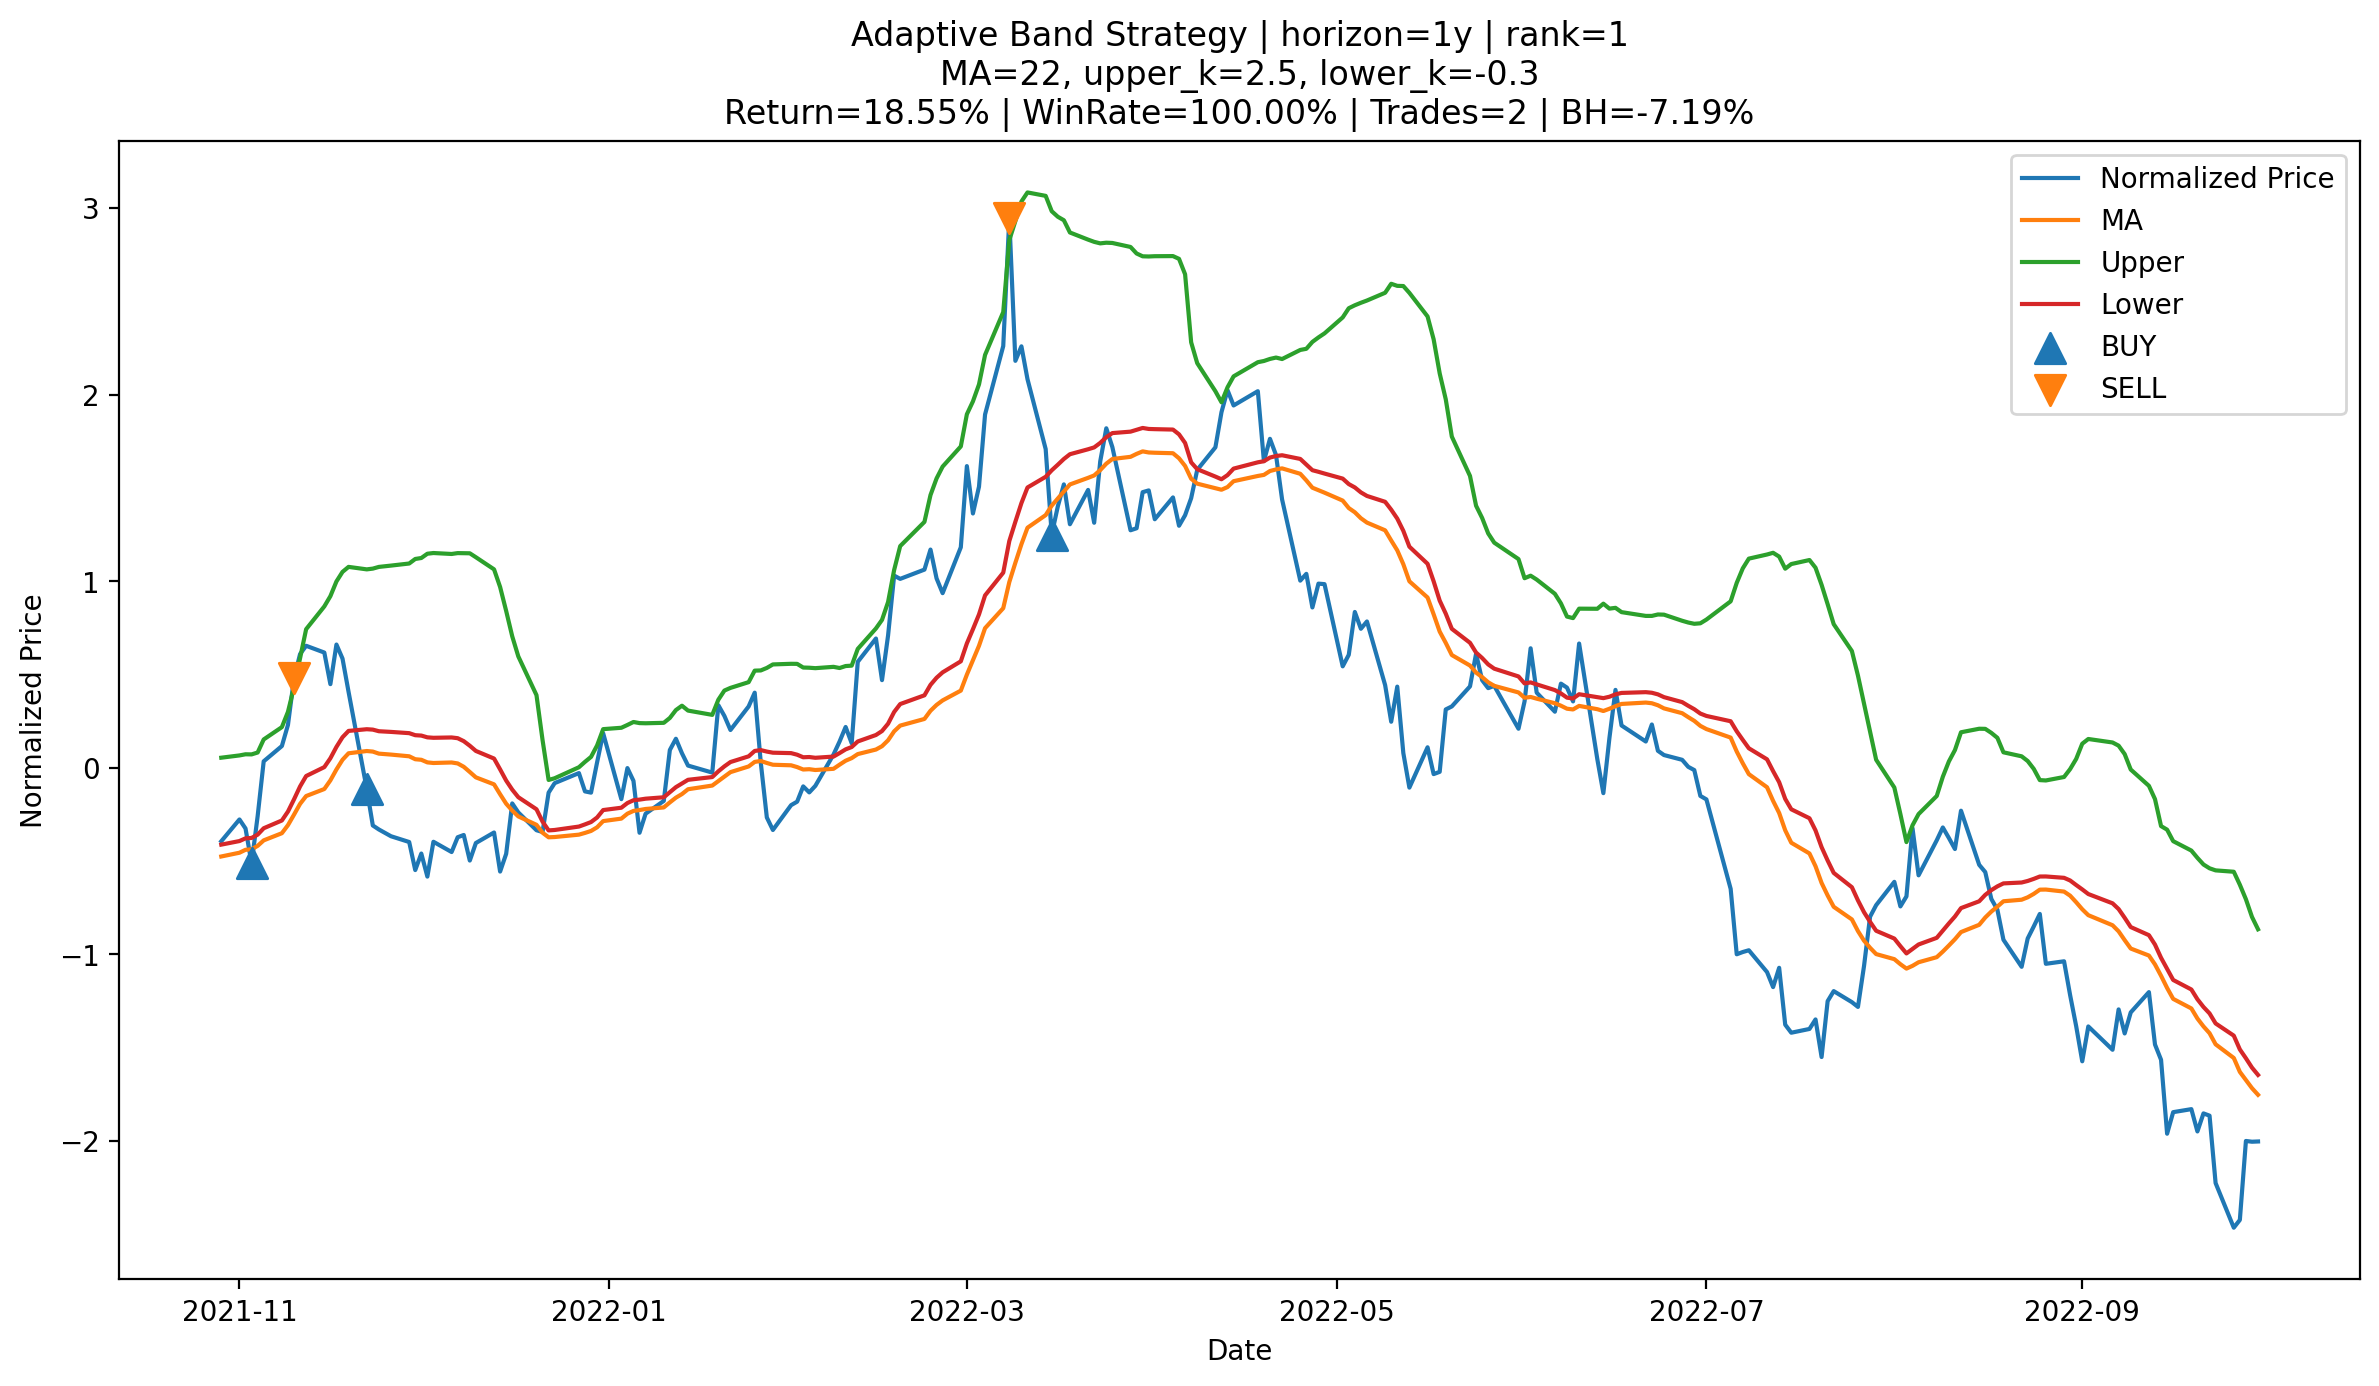
\includegraphics[width=\textwidth]{../../figures/adaptive_band_strategy/1y/1y_rank01_ma22_uk2.5_lk-0.3.png}
    \end{column}
  \end{columns}
\end{frame}

% ── Slide 6: Strategy 2 ──────────────────────────────────────────────────────
\begin{frame}{Strategy 2: Moving-Average Crossover}
  \begin{columns}[T]
    \begin{column}{0.40\textwidth}
      \small
      \textbf{Signal type: continuous}
      \vspace{0.4em}
      \begin{itemize}
        \item Short-window MA compared against long-window MA
        \item Positive spread: uptrend; negative spread: downtrend
        \item Score captures direction and magnitude of the gap
        \item Buy: short MA crosses above long MA
        \item Sell: short MA crosses below long MA
      \end{itemize}
    \end{column}
    \begin{column}{0.57\textwidth}
      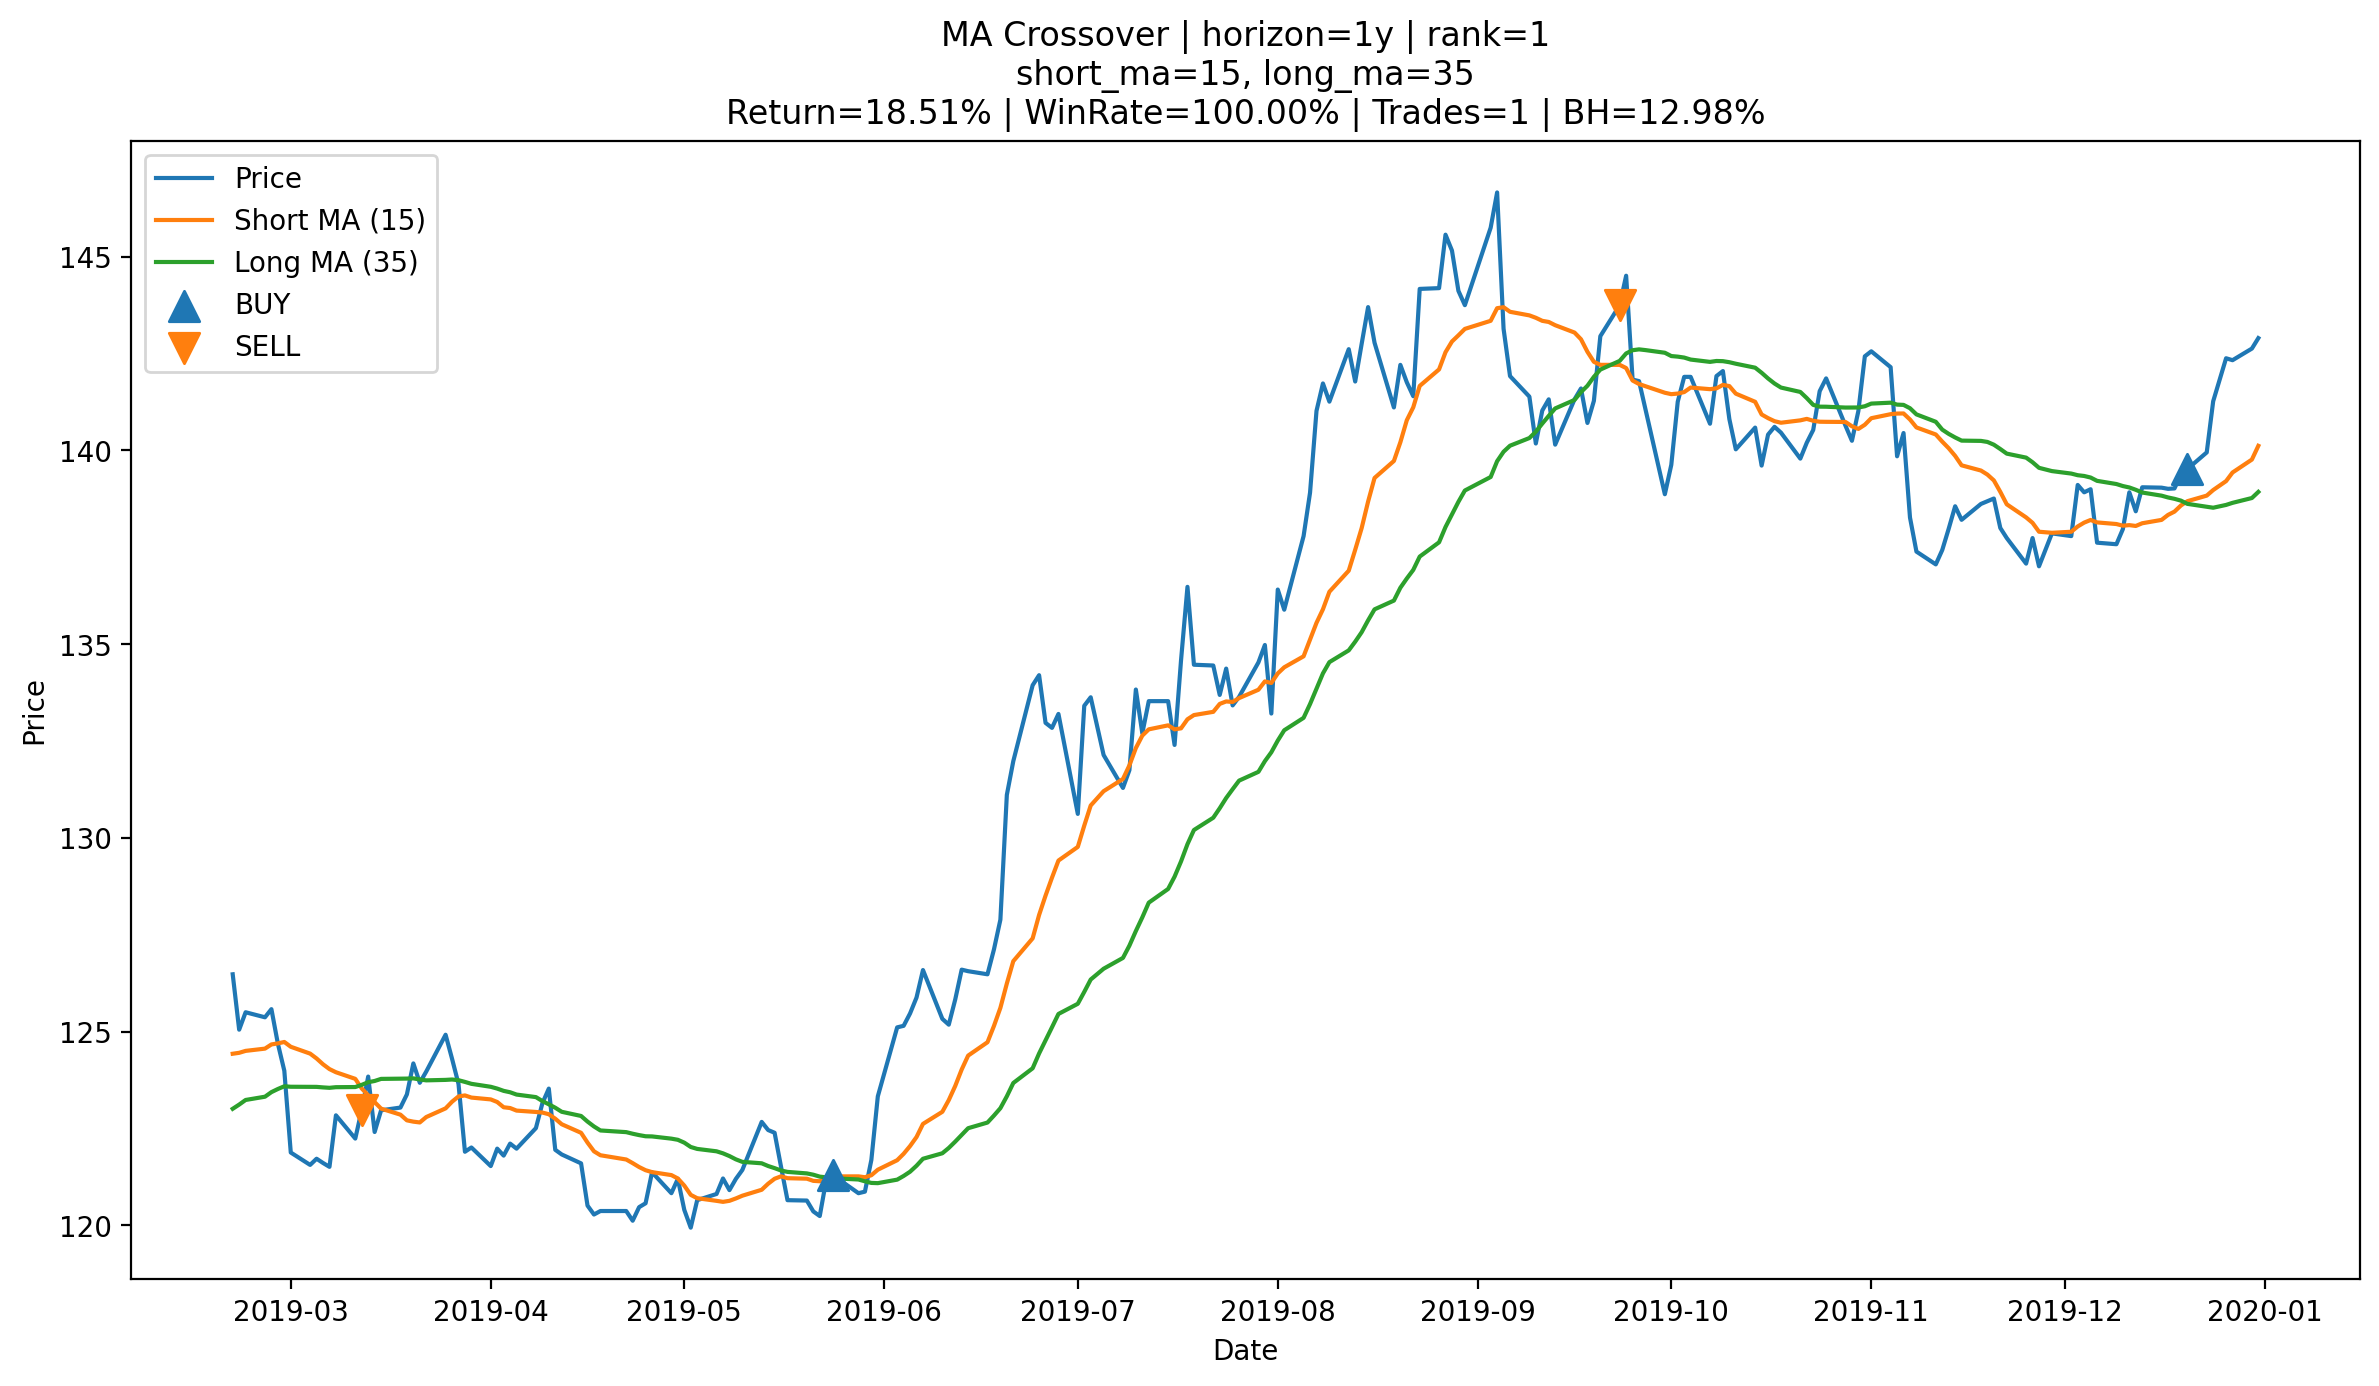
\includegraphics[width=\textwidth]{../../figures/ma_crossover/1y/1y_rank01_sma15_lma35.png}
    \end{column}
  \end{columns}
\end{frame}

% ── Slide 7: Strategy 3 ──────────────────────────────────────────────────────
\begin{frame}{Strategy 3: Adaptive Volatility Band}
  \begin{columns}[T]
    \begin{column}{0.40\textwidth}
      \small
      \textbf{Signal type: continuous}
      \vspace{0.4em}
      \begin{itemize}
        \item Volatility proxy from high-low-close range
        \item Bands placed relative to rolling volatility level
        \item Score reflects current volatility regime position
        \item High-vol breakouts and low-vol compressions produce distinct signals
        \item Complementary to price-band strategies
      \end{itemize}
    \end{column}
    \begin{column}{0.57\textwidth}
      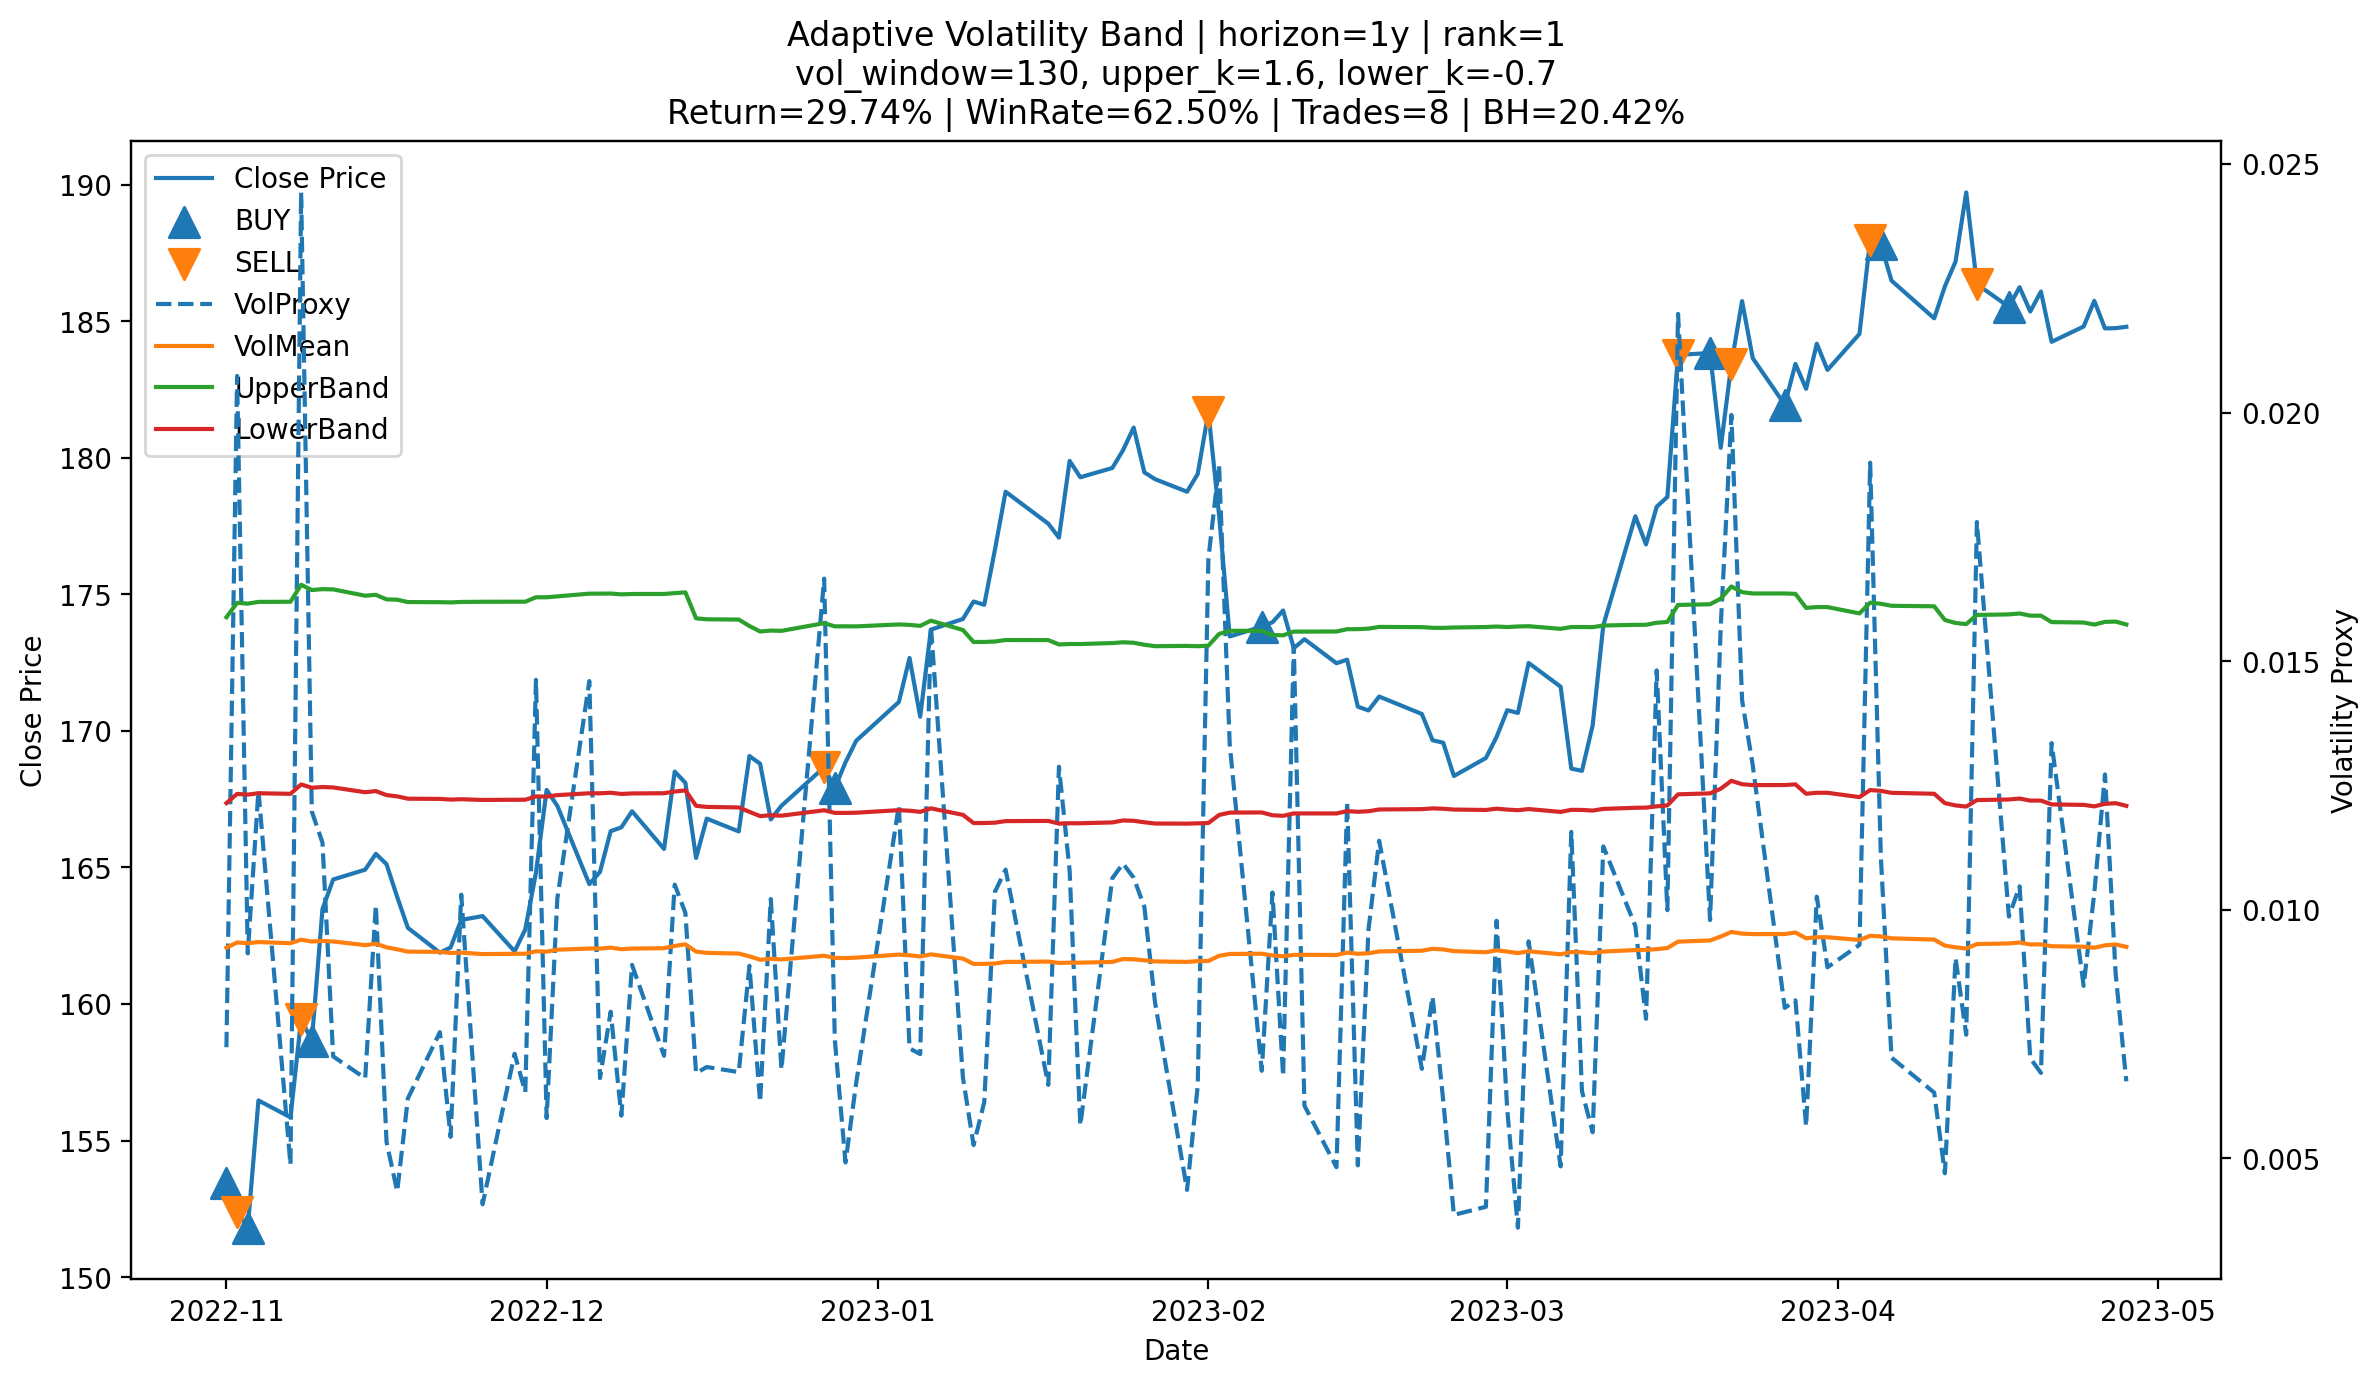
\includegraphics[width=\textwidth]{../../figures/adaptive_volatility_band_strategy/1y/1y_rank01_vw130_uk1.6_lk-0.7.png}
    \end{column}
  \end{columns}
\end{frame}

% ── Slide 8: Strategy 4 ──────────────────────────────────────────────────────
\begin{frame}{Strategy 4: Fear-Greed Candle-Volume}
  \begin{columns}[T]
    \begin{column}{0.40\textwidth}
      \small
      \textbf{Signal type: event-style}
      \vspace{0.4em}
      \begin{itemize}
        \item Fires only when candle body size \textbf{and} volume spike simultaneously
        \item Captures extreme sentiment: large directional move confirmed by activity
        \item Rare by design; most days produce no signal
        \item Qualitatively different from the three continuous strategies
        \item Adds a sparse basis vector to matrix \(A\)
      \end{itemize}
    \end{column}
    \begin{column}{0.57\textwidth}
      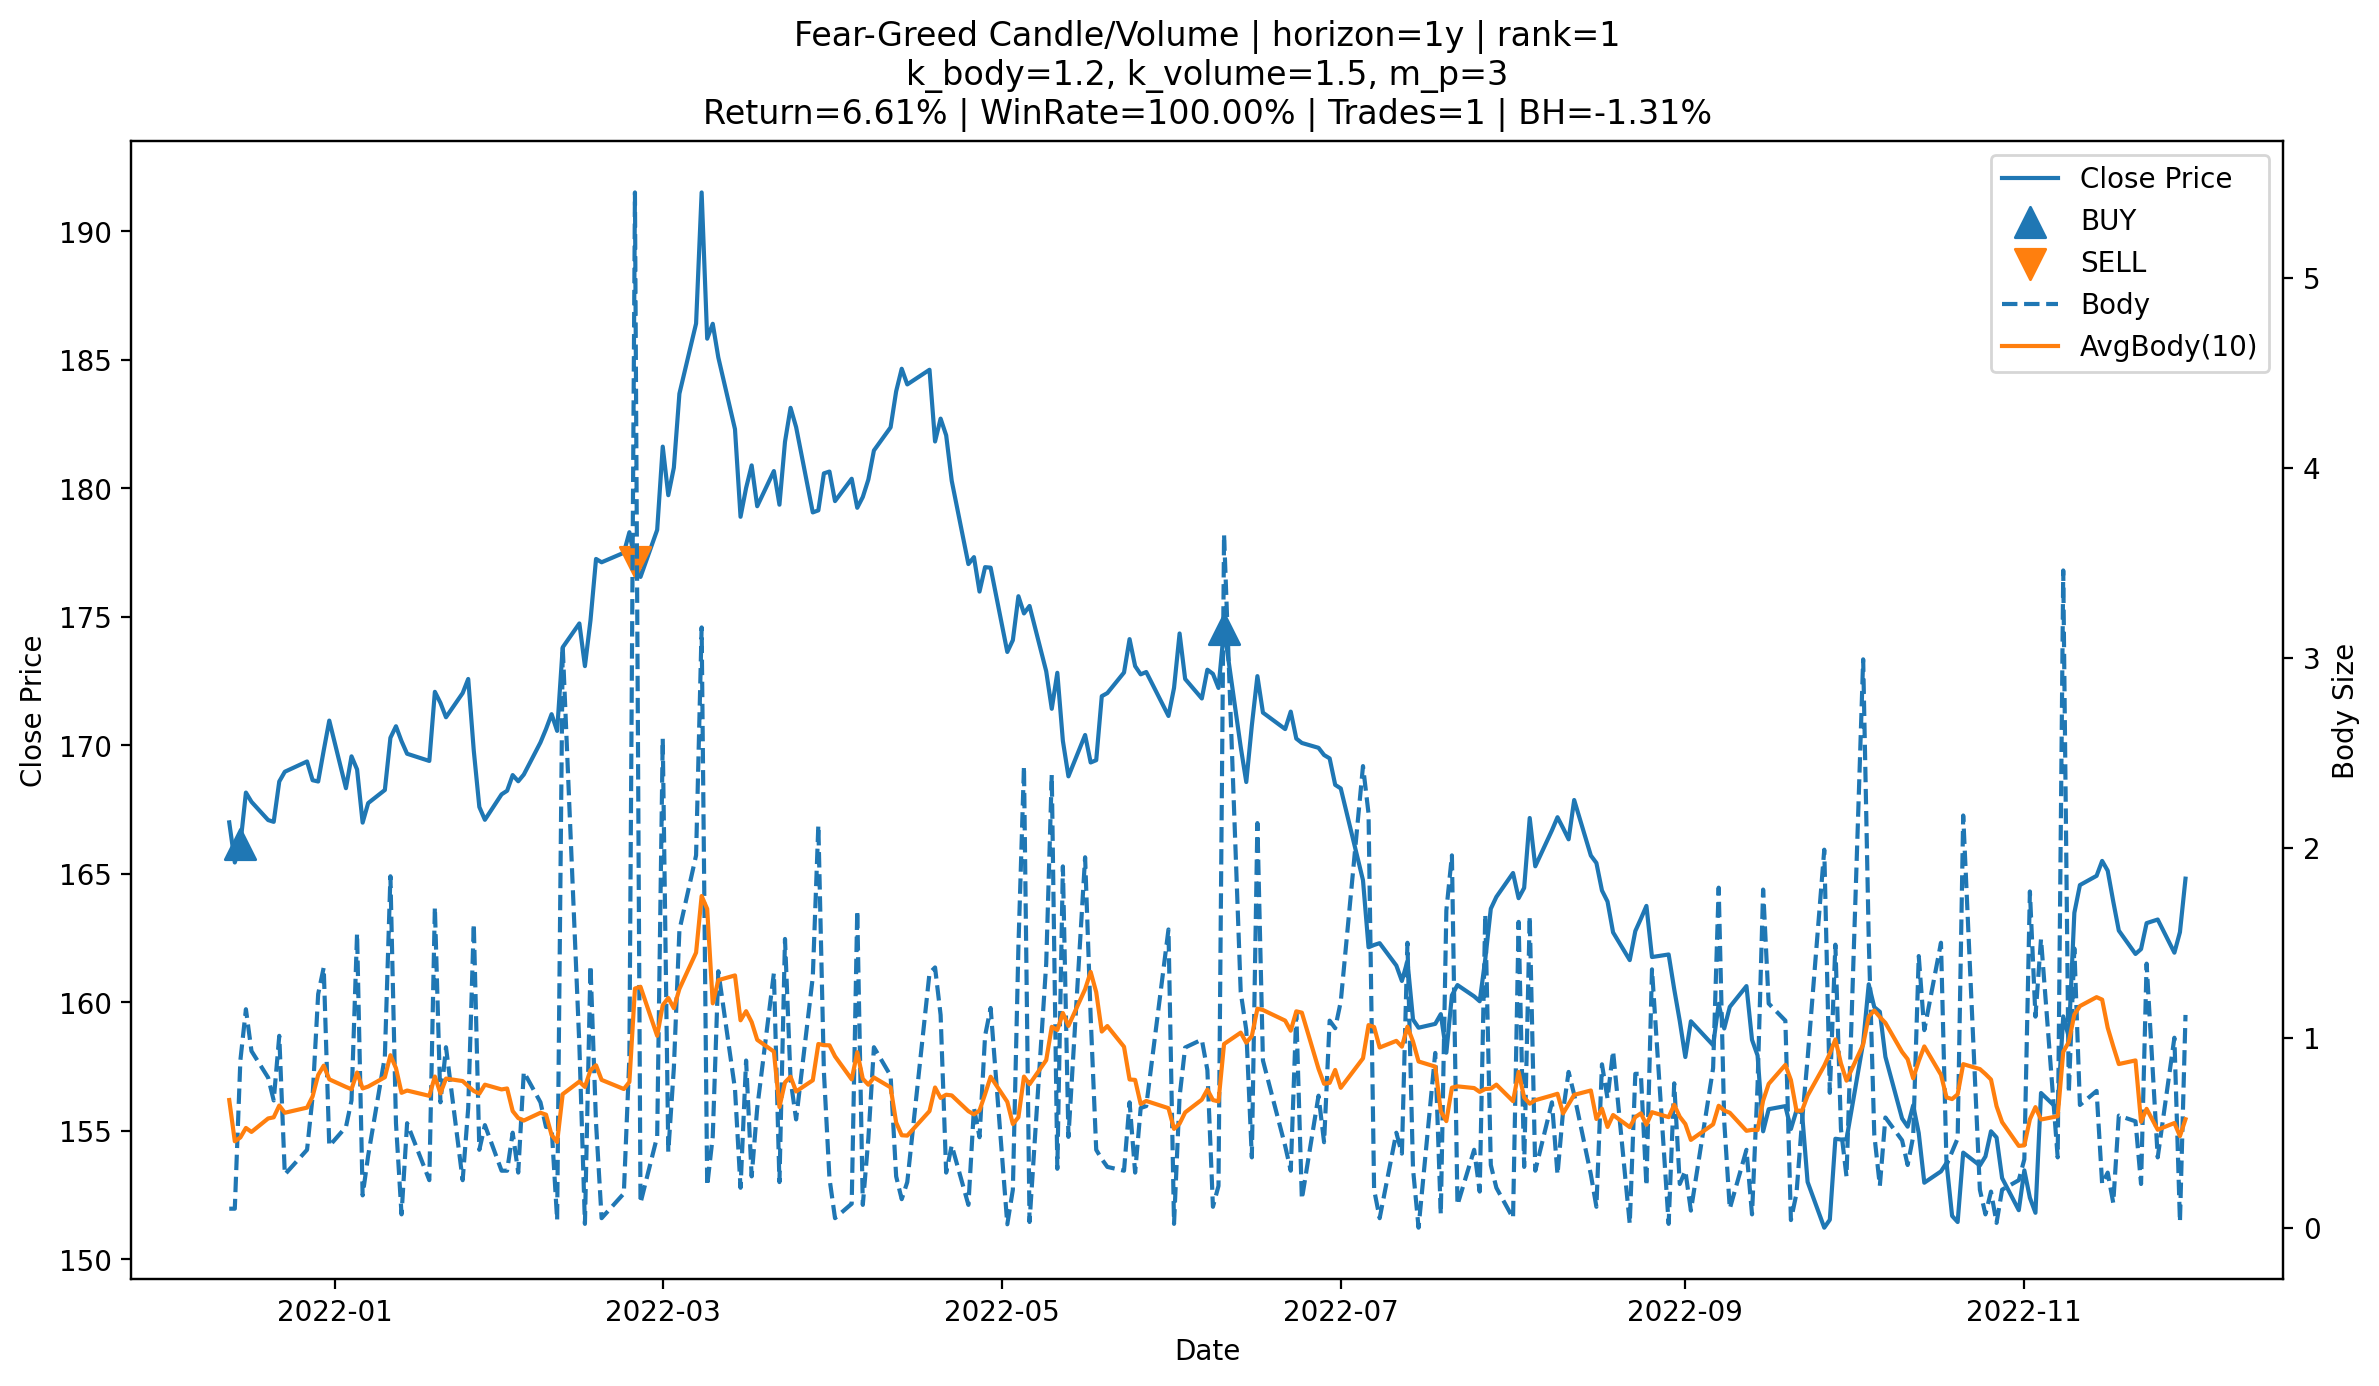
\includegraphics[width=\textwidth]{../../figures/fear_greed_candle_volume_strategy/1y/1y_rank01_kb1.2_kv1.5_mp3.png}
    \end{column}
  \end{columns}
\end{frame}

% ── Slide 9: Parameters as Functions ────────────────────────────────────────
\begin{frame}{Turning Parameters into Signals}
  Each strategy family has its own parameters. After optimization, the best
  parameters define a concrete signal function for that anchor.

  \vspace{0.4em}
  \textbf{Example: anchor date 2021-12-31}

  \vspace{0.3em}
  \textbf{Strategy 1 — Adaptive Band} \hfill (MA=65, upper\_k=0.0, lower\_k=0.6)
  \[
    s_{\text{band}}(t) = \frac{P_t - \text{MA}_{65}(t)}{\sigma_{65}(t)},
    \quad \text{buy signal when } s_{\text{band}}(t) < 0.6
  \]

  \vspace{0.2em}
  \textbf{Strategy 2 — MA Crossover} \hfill (short=60, long=65)
  \[
    s_{\text{ma}}(t) = \text{MA}_{60}(t) - \text{MA}_{65}(t),
    \quad \text{buy signal when } s_{\text{ma}}(t) > 0
  \]

  \vspace{0.4em}
  \begin{itemize}
    \item Parameters are re-optimized at every anchor date (monthly)
    \item Each anchor produces a different function adapted to recent market behavior
    \item The score value on any day becomes one entry in matrix \(A\)
  \end{itemize}
\end{frame}

% ── Slide 10: Stage A Results ────────────────────────────────────────────────
\begin{frame}{Stage A: What Happens with One Strategy at a Time?}
  \small
  Hold 130 days $\cdot$ 1-month parameter update $\cdot$ rank-1 parameters per anchor

  \vspace{0.4em}
  \begin{tabular}{lrrrrr}
    \toprule
    Year & B\&H & Adap.Band & MA Cross & Adap.Vol & Fear-Greed \\
    \midrule
    2020 & +23.9\% & +4.4\% & +5.2\% & +5.8\% & $\approx$0\% \\
    2021 & $-$6.2\%  & +0.3\% & $-$0.2\% & +0.9\% & $\approx$0\% \\
    2022 & +0.8\%  & $-$0.9\% & $-$3.0\% & $-$2.1\% & $\approx$0\% \\
    2023 & +11.8\% & +1.5\% & +0.9\% & +2.1\% & $\approx$0\% \\
    2024 & +27.0\% & +5.9\% & +6.3\% & +10.6\% & $\approx$0\% \\
    \bottomrule
  \end{tabular}

  \vspace{0.5em}
  \begin{itemize}
    \item Each strategy alone captures only a \textbf{fraction} of the market move
    \item Exposure is low (21--46\%): the strategy sits out most days
    \item Fear-Greed: after removing look-ahead bug, GLD rarely triggers ($\approx$0\% exposure)
  \end{itemize}
\end{frame}

% ── Slide 11: Stage B — Matrix A ─────────────────────────────────────────────
\begin{frame}{Stage B: Combining Strategies — Matrix A}
  Single strategies each capture a partial signal.
  \textbf{Can combining them do better?}

  \vspace{0.5em}
  Define the design matrix \(A\) where each column is one strategy score:
  \[
    A \;=\;
    \begin{pmatrix}
      s_1(t_1) & s_2(t_1) & s_3(t_1) & s_4(t_1) \\
      s_1(t_2) & s_2(t_2) & s_3(t_2) & s_4(t_2) \\
      \vdots   & \vdots   & \vdots   & \vdots   \\
      s_1(t_n) & s_2(t_n) & s_3(t_n) & s_4(t_n)
    \end{pmatrix}
  \]

  \vspace{0.3em}
  Find weights \(\mathbf{x} \geq 0\) (long-only) that maximize realized return \(y\):
  \[
    \max_{\mathbf{x} \geq 0,\; \mathbf{1}^\top \mathbf{x} = 1}
    \quad y(\mathbf{x}) \;=\; \text{portfolio return using combined signal } A\mathbf{x}
  \]

  \vspace{0.3em}
  \textbf{Objective 1}: constrained optimization over the strategy space.\\
  Parameters re-optimized at each anchor date (rolling walk-forward).
\end{frame}

% ── Slide 13: Stage B — Optimizer Example ────────────────────────────────────
\begin{frame}{Stage B: What Did the Optimizer Actually Find?}
  \textbf{Anchor: 2021-12-31} — selection period return vs.\ buy-and-hold: \textbf{+10.2\% vs $-$6.2\%}

  \vspace{0.4em}
  Long-only weight optimization over the 4 strategy signals:
  \[
    \hat{s}(t) \;=\; \underbrace{0.45}_{\text{Adaptive Band}} \cdot s_{\text{band}}(t)
              \;+\; \underbrace{0.00}_{\text{MA Cross}} \cdot s_{\text{ma}}(t)
              \;+\; \underbrace{0.55}_{\text{Adap.Vol}} \cdot s_{\text{vol}}(t)
              \;+\; \underbrace{0.00}_{\text{Fear-Greed}} \cdot s_{\text{fg}}(t)
  \]

  \vspace{0.4em}
  \begin{itemize}
    \item Two strategies dominate: Adaptive Band (45\%) and Adaptive Vol (55\%)
    \item MA Crossover and Fear-Greed received zero weight — optimizer excluded them
    \item This mirrors Lasso-style selection: only the most informative signals survive
    \item Standalone returns in selection period: Band=+10.0\%, Vol=+10.1\%, MA=$-$5.6\%
  \end{itemize}
\end{frame}

% ── Slide 14: Stage B — Ensemble Results ─────────────────────────────────────
\begin{frame}{Stage B: Ensemble Results}
  \small
  Hold 130 days $\cdot$ 1-month update $\cdot$ long-only weight re-optimization per anchor

  \vspace{0.4em}
  \begin{tabular}{lrrrr}
    \toprule
    Year & B\&H & Stage A (best single) & Stage B (ensemble) & Change \\
    \midrule
    2020 & +23.9\% & +4.4\% & +6.4\% & $\uparrow$ \\
    2021 & $-$6.2\%  & +0.3\% & +0.3\% & $\sim$ \\
    2022 & +0.8\%  & $-$0.9\% & $-$2.3\% & $\downarrow$ \\
    2023 & +11.8\% & +1.6\% & +2.0\% & $\uparrow$ \\
    2024 & +27.0\% & +5.9\% & +8.0\% & $\uparrow$ \\
    \bottomrule
  \end{tabular}

  \vspace{0.5em}
  \begin{itemize}
    \item Ensemble beats single strategy in 3/5 years, but margin is small
    \item 2022: ensemble \emph{worse} ($-$2.3\% vs $-$0.9\%) --- diversification hurts in whipsaw markets
    \item \textbf{Weights are fixed after optimization — cannot adapt to current market regime}
  \end{itemize}
\end{frame}

% ── Slide 15: What Stage B Cannot Do ─────────────────────────────────────────
\begin{frame}{What Stage B Cannot Do}
  Stage B finds the best \emph{historical} weight vector \(\mathbf{x}\).\\
  But the market changes — the optimal combination today may differ from last month.

  \vspace{0.5em}
  \textbf{The missing step:}
  \[
    \text{learn how to combine signals to predict } \textbf{future} \text{ return}
  \]

  \vspace{0.5em}
  \begin{tabular}{lll}
    \toprule
    & Stage B & Stage C \\
    \midrule
    Question    & best historical weights? & what predicts future return? \\
    Method      & constrained optimization & supervised learning \\
    Signal use  & combine realized returns & use current scores as features \\
    Adaptation  & fixed per anchor         & model selected per anchor \\
    \bottomrule
  \end{tabular}
\end{frame}

% ── Slide 16: Stage C — Expanded Space ───────────────────────────────────────
\begin{frame}{Stage C: Expanding the Strategy Space}
  \textbf{Objective 2}: treat strategy scores as \emph{features} for a supervised model.

  \vspace{0.4em}
  Expand from 4 to \textbf{40 basis columns}:
  \[
    A \in \mathbb{R}^{n \times 40}
    \quad \text{(top 10 parameter sets per strategy family)}
  \]

  \vspace{0.3em}
  This mirrors the class model-selection exercise:
  \[
    \text{many basis functions} \;\longrightarrow\; \text{select useful structure}
  \]

  \vspace{0.4em}
  Four linear models compared:
  \[
    \text{OLS} \quad \text{Ridge} \quad \text{Lasso} \quad \text{Elastic Net}
  \]

  \vspace{0.3em}
  Model selection criterion: \textbf{time-series cross-validated MSE} (no look-ahead).
\end{frame}

% ── Slide 17: Stage C — Forward Validation ───────────────────────────────────
\begin{frame}{Stage C: Forward Validation Design}
  \begin{columns}[T]
    \begin{column}{0.50\textwidth}
      \textbf{Anchor-date setup}
      \vspace{0.4em}
      \begin{itemize}
        \item Monthly anchor dates: 2020--2024
        \item \textbf{Selection period}: 1 year before anchor
        \begin{itemize}
          \item fit model, pick best by CV-MSE
        \end{itemize}
        \item \textbf{Evaluation period}: after anchor
        \begin{itemize}
          \item apply frozen model to unseen data
        \end{itemize}
        \item Model re-fitted at each new anchor
      \end{itemize}
    \end{column}
    \begin{column}{0.47\textwidth}
      \vspace{1.5em}
      \[
        \underbrace{\longleftarrow\text{1 year}\longrightarrow}_{\text{selection}}
        \Big|_{\text{anchor}}
        \underbrace{\longrightarrow}_{\text{evaluation}}
      \]
      \vspace{0.8em}
      \small
      The model never sees future data during fitting.\\[0.5em]
      This separates model discovery from forward validation.
    \end{column}
  \end{columns}
\end{frame}

% ── Slide 18: Stage C — Prediction to Weight ─────────────────────────────────
\begin{frame}{Stage C: From Prediction to Portfolio Weight}
  The model outputs a predicted future cumulative return \(\hat{y}_t\).

  \vspace{0.5em}
  Convert to a long-only portfolio weight:
  \[
    w_t \;=\; \operatorname{clip}\!\left(\frac{\hat{y}_t}{s},\; 0,\; 1\right)
  \]
  where \(s\) is a quantile-based scale factor from the selection period.

  \vspace{0.5em}
  Execute via rolling \textbf{tranches} (small independent positions):
  \begin{itemize}
    \item Each day: compute signal, open one tranche at weight \(w_t\)
    \item Hold for fixed horizon (45 or 130 days), then close
    \item Gross exposure = average of all open tranches at any moment
  \end{itemize}

  \vspace{0.4em}
  \textbf{Key property}: when the model is confident (\(\hat{y}_t\) large), exposure rises.\\
  When uncertain (\(\hat{y}_t \approx 0\)), exposure falls naturally.
\end{frame}

% ── Slide 19: Stage C Model Example ──────────────────────────────────────────
\begin{frame}{Stage C: What Does the Chosen Model Look Like?}
  \textbf{Anchor: 2021-11-30} — OLS selected, horizon=130 days

  \vspace{0.3em}
  From 40 basis columns, the top contributing features (by absolute coefficient):

  \vspace{0.3em}
  \small
  \begin{tabular}{llr}
    \toprule
    Feature & Strategy family & Coefficient \\
    \midrule
    \texttt{ma\_crossover\_rank07}       & MA Crossover   & $-0.212$ \\
    \texttt{adaptive\_band\_rank05}      & Adaptive Band  & $+0.099$ \\
    \texttt{adaptive\_band\_rank06}      & Adaptive Band  & $+0.097$ \\
    \texttt{adaptive\_band\_rank03}      & Adaptive Band  & $-0.075$ \\
    \texttt{adaptive\_band\_rank04}      & Adaptive Band  & $-0.073$ \\
    \texttt{ma\_crossover\_rank10}       & MA Crossover   & $+0.071$ \\
    $\vdots$ & $\vdots$ & $\vdots$ \\
    \bottomrule
  \end{tabular}

  \normalsize
  \vspace{0.4em}
  \begin{itemize}
    \item 28 of 40 features nonzero — OLS uses the full correlated space
    \item Model mixes \emph{ranks within a strategy}, not just strategies
    \item \(\hat{y}_t = \beta_0 + \sum_j \beta_j A_{tj}\) becomes weight \(w_t = \operatorname{clip}(\hat{y}_t/s,\,0,\,1)\)
  \end{itemize}
\end{frame}

% ── What Exposure Really Means ───────────────────────────────────────────────
\begin{frame}{What ``Exposure'' Means in Each Stage}
  \small
  \textbf{Stage A \& B} — signal is binary: each day is either fully in (100\%) or fully out (0\%).
  \[
    \text{Exposure}_{A,B} = \frac{\text{\# days in market}}{\text{total days}}
    \quad \text{(time-averaged binary — not a real weight)}
  \]

  \textbf{Stage C} — model outputs a continuous daily weight \(w_t \in [0,\,1]\):
  \[
    w_t = \operatorname{clip}\!\left(\frac{\hat{y}_t}{s},\; 0,\; 1\right),
    \qquad
    \text{Exposure}_C = \frac{1}{T}\sum_t w_t
    \quad \text{(true capital weight)}
  \]

  When the model is confident, \(w_t\) is large. When uncertain, \(w_t \to 0\).
  This is real variable exposure, not just in/out frequency.

  \vspace{0.4em}
  \textbf{Capital Efficiency = Return $\div$ Avg.\ Exposure} \hfill (2024, h130 vs h45)

  \vspace{0.3em}
  \begin{tabular}{lrrr}
    \toprule
    & Return & Avg.\ Exposure & Efficiency \\
    \midrule
    Buy-and-Hold           & +27.0\% & 100\% & +27\% \\
    Stage C, hold 130 days & +16.4\% &  65\% & +25\% \\
    Stage C, hold 45 days  & +25.2\% &  78\% & \textbf{+32\%} \\
    \bottomrule
  \end{tabular}

  \vspace{0.3em}
  h45 Stage C efficiency \textbf{exceeds} B\&H in 2024. Idle capital can be deployed elsewhere.
\end{frame}

% ── Slide 21: Three-Stage Comparison — KEY SLIDE ─────────────────────────────
\begin{frame}{Three-Stage Comparison: A vs B vs C}
  \small
  Hold 130 days $\cdot$ 1-month update $\cdot$ \textbf{Return / Avg.\ Exposure}

  \vspace{0.4em}
  \begin{tabular}{lrrrrr}
    \toprule
    Year & B\&H & A: Single Signal & B: Ensemble & C: ML-Guided \\
    \midrule
    2020 & +23.9\% & +4.4\% / 27\% & +6.4\% / 32\% & \textbf{+10.9\%} / 57\% \\
    2021 & $-$6.2\%  & +0.3\% / 25\% & +0.3\% / 25\% & \textbf{+0.8\%} / 29\% \\
    2022 & +0.8\%  & $-$0.9\% / 46\% & $-$2.3\% / 42\% & \textbf{$-$0.2\%} / 31\% \\
    2023 & +11.8\% & +1.6\% / 25\% & +2.0\% / 23\% & \textbf{+4.0\%} / 32\% \\
    2024 & +27.0\% & +5.9\% / 21\% & +8.0\% / 29\% & \textbf{+16.4\%} / 65\% \\
    \bottomrule
  \end{tabular}

  \vspace{0.5em}
  \begin{itemize}
    \item C outperforms A and B in \textbf{every year} on both return and exposure efficiency
    \item 2024: A(+5.9\%) $\to$ B(+8.0\%) $\to$ \textbf{C(+16.4\%)} — clear step-up at each stage
    \item ML-Guided learns \emph{when} and \emph{how much} to bet, not just which strategy
  \end{itemize}
\end{frame}

% ── Slide 21: Update Frequency — Hold 130 Days ───────────────────────────────
\begin{frame}{How Often Should the Model Update? — Hold 130 Days}
  \small
  Stage C $\cdot$ Ret / Avg.\ Exposure

  \vspace{0.4em}
  \begin{tabular}{lrrrrr}
    \toprule
    Year & B\&H & 1M & 2M & 3M & 6M \\
    \midrule
    2020 & +23.9\% & +10.9\% / 57\% & +10.2\% / 57\% & +9.6\% / 51\% & +9.7\% / 50\% \\
    2021 & $-$6.2\%  & +0.8\% / 29\% & +0.3\% / 35\% & +0.6\% / 28\% & $-$0.7\% / 49\% \\
    2022 & +0.8\%  & $-$0.2\% / 31\% & +0.9\% / 35\% & $-$0.8\% / 33\% & $-$1.7\% / 44\% \\
    2023 & +11.8\% & +4.0\% / 32\% & +4.1\% / 23\% & +3.8\% / 40\% & +3.4\% / 15\% \\
    2024 & +27.0\% & \textbf{+16.4\%} / 65\% & +13.9\% / 60\% & +11.1\% / 53\% & +5.5\% / 36\% \\
    \bottomrule
  \end{tabular}

  \vspace{0.5em}
  \begin{itemize}
    \item \textbf{1M consistently best}: fastest adaptation captures regime shifts
    \item 2024: 1M captures the full bull run; 6M misses most of it (+5.5\%)
    \item More frequent updates require more compute — but pay off significantly
  \end{itemize}
\end{frame}

% ── Slide 22: Update Frequency — Hold 45 Days ────────────────────────────────
\begin{frame}{How Often Should the Model Update? — Hold 45 Days}
  \small
  Stage C $\cdot$ Ret / Avg.\ Exposure

  \vspace{0.4em}
  \begin{tabular}{lrrrrr}
    \toprule
    Year & B\&H & 1M & 2M & 3M & 6M \\
    \midrule
    2020 & +23.9\% & +17.4\% / 72\% & +16.5\% / 71\% & +13.7\% / 64\% & +13.3\% / 63\% \\
    2021 & $-$6.2\%  & +1.5\% / 35\% & +1.8\% / 37\% & +1.2\% / 34\% & $-$1.2\% / 49\% \\
    2022 & +0.8\%  & $-$0.6\% / 37\% & +1.3\% / 42\% & $-$0.6\% / 38\% & $-$2.5\% / 51\% \\
    2023 & +11.8\% & +2.5\% / 44\% & +3.7\% / 34\% & +0.9\% / 50\% & +3.8\% / 24\% \\
    2024 & +27.0\% & \textbf{+25.2\%} / 78\% & +19.8\% / 73\% & +16.2\% / 66\% & +11.0\% / 52\% \\
    \bottomrule
  \end{tabular}

  \vspace{0.5em}
  \begin{itemize}
    \item 1M remains the strongest — same conclusion across both horizons
    \item h45 captures bull markets more aggressively (2024: +25.2\% vs h130: +16.4\%)
    \item Shorter hold = faster signal turnover = better regime adaptation
  \end{itemize}
\end{frame}

% ── Slide 23: Hold Horizon Comparison ────────────────────────────────────────
\begin{frame}{Hold Horizon: 45 Days vs 130 Days}
  \small
  Stage C $\cdot$ 1-month update $\cdot$ Ret / Exposure / Efficiency

  \vspace{0.4em}
  \begin{tabular}{lrcc}
    \toprule
    Year & B\&H & Hold 130 days & Hold 45 days \\
    \midrule
    2020 & +23.9\% / +24\% eff & +10.9\% / 57\% / +19\% & \textbf{+17.4\%} / 72\% / +24\% \\
    2021 & $-$6.2\% / $-$6\% eff  & \textbf{+0.8\%} / 29\% / +3\% & +1.5\% / 35\% / +4\% \\
    2022 & +0.8\% / +1\% eff   & \textbf{$-$0.2\%} / 31\% / $-$1\% & $-$0.6\% / 37\% / $-$2\% \\
    2023 & +11.8\% / +12\% eff & \textbf{+4.0\%} / 32\% / +12\% & +2.5\% / 44\% / +6\% \\
    2024 & +27.0\% / +27\% eff & +16.4\% / 65\% / +25\% & \textbf{+25.2\%} / 78\% / \textbf{+32\%} \\
    \bottomrule
  \end{tabular}

  \vspace{0.4em}
  \begin{itemize}
    \item \textbf{h45} captures bull markets better (2020, 2024) — faster turnover
    \item \textbf{h130} more stable in flat/bear markets (2022, 2023)
    \item h45 efficiency in 2024 (\textbf{+32\%}) exceeds B\&H (+27\%) — better return per capital deployed
  \end{itemize}
\end{frame}

% ── Slide 25: Live Signal Example ────────────────────────────────────────────
\begin{frame}{Stage C in Production: Live Signal (April 25, 2026)}
  \textbf{Signal generated daily at 13:00 PDT by Raspberry Pi --- as of 2026-04-24}

  \vspace{0.5em}
  \begin{tabular}{ll}
    \toprule
    Field & Value \\
    \midrule
    Symbol                       & GLD \\
    As-of Date                   & 2026-04-24 \\
    Close Price                  & \$432.97 \\
    \textbf{Signal}              & \textbf{BUY (strong)} \\
    Target Weight                & 1.00 \quad (full position) \\
    Predicted Return (130 days)  & +55.6\% \\
    Active Model                 & Ridge \\
    Active Anchor                & 2026-03-31 \\
    Dominant Strategy Family     & MA Crossover \\
    \bottomrule
  \end{tabular}

  \vspace{0.5em}
  \begin{itemize}
    \item Anchor updates monthly --- today uses the \textbf{most recent anchor} (2026-03-31)
    \item Ridge selected by CV-MSE from \{OLS, Ridge, Lasso, ElasticNet\}
    \item Signal pushed to GitHub automatically; order execution via Alpaca (paper trading)
  \end{itemize}
\end{frame}

% ── Slide 26: What's Next ─────────────────────────────────────────────────────
\begin{frame}{What's Next? — Priorities}
  \small
  \textbf{1. Multi-Asset Expansion} \hfill \textit{immediate — data already collected}
  \begin{itemize}
    \item Apply framework to BRK.B, oil, copper, equities
    \item Deploy idle GLD capital into other assets when GLD exposure is low
  \end{itemize}

  \vspace{0.4em}
  \textbf{2. Regime-Aware Exposure Control} \hfill \textit{short-term}
  \begin{itemize}
    \item Add a second-layer signal: \emph{is the market currently predictable?}
    \item Reduce exposure globally during high-uncertainty regimes
  \end{itemize}

  \vspace{0.4em}
  \textbf{3. Nonlinear Model Selection via SINDy} \hfill \textit{research}
  \begin{itemize}
    \item Expand library: \(\Theta(A) = [s_i,\; s_i^2,\; s_i s_j,\; \dots]\)
    \item Sparse regression selects only the terms that matter
  \end{itemize}

  \vspace{0.4em}
  \textbf{4. Hierarchical Strategy Structure} \hfill \textit{research}
  \begin{itemize}
    \item Direction signals $\to$ timing signals: each layer applies a nonlinear transform
  \end{itemize}
\end{frame}

% ── Slide 25: Conclusion ──────────────────────────────────────────────────────
\begin{frame}{Conclusion}
  \small
  \begin{block}{Main Finding}
    Treating trading strategy outputs as basis functions creates a valid,
    predictive strategy space. ML model selection over that space substantially
    outperforms both single-strategy and ensemble approaches.
  \end{block}

  \vspace{0.3em}
  \begin{tabular}{ll}
    \toprule
    Stage & Key Takeaway \\
    \midrule
    A: Single Signal  & Exposure 21--46\%; captures small fraction of market move \\
    B: Ensemble       & Diversification alone does not improve prediction \\
    C: ML-Guided      & Learns \emph{when} to be exposed; 2024: $\times$2.0 vs B, $\times$2.8 vs A \\
    \bottomrule
  \end{tabular}

  \vspace{0.4em}
  \footnotesize
  \textbf{Mini Project Team:}
  Alejandro Menacho, Ashmeet Singh, Claire Wang, Thomas Tran,
  Matthew Aguirre, Sophia Wei, Jack, Stephen\\[0.2em]
  Stage A--B developed jointly with Jack, Stephen, Sophia, and Claire.\\[0.15em]
  Live trading pipeline on Raspberry Pi: Jack and Stephen.
\end{frame}

% ── Q&A Divider ───────────────────────────────────────────────────────────────
\begin{frame}{}
  \begin{center}
    \vspace{2em}
    {\Large\color{qNavy}\textbf{Questions?}}\\[1.5em]
    \small
    \begin{tabular}{ll}
      Appendix A & Grid Search Parameter Ranges \\
      Appendix B & Stage C Hyperparameter Search (CV design) \\
      Appendix C & Performance Excluding 2024 \\
      Appendix D & Three-Stage Comparison --- Hold 45 Days \\
      Appendix E & Transaction Costs \\
    \end{tabular}
  \end{center}
\end{frame}

% ═══════════════════════════════════════════════════════════════════════════
%  APPENDIX
% ═══════════════════════════════════════════════════════════════════════════

% ── Appendix A: Grid Search — Strategy Parameters ────────────────────────────
\begin{frame}{Appendix A: Grid Search — Strategy Parameter Ranges}
  \small
  Each strategy optimized independently over its representative horizon.

  \vspace{0.4em}
  \begin{tabular}{llll}
    \toprule
    Strategy & Horizon & Parameter & Search Range \\
    \midrule
    \multirow{3}{*}{Adaptive Band}
      & \multirow{3}{*}{1y}
      & \texttt{ma\_window}  & \{5, 10, 22, 65, 130, 260\} (horizon-filtered) \\
      && \texttt{upper\_k}   & $-3.0$ to $+3.0$, step $0.1$ \quad (61 values) \\
      && \texttt{lower\_k}   & $-3.0$ to $+3.0$, step $0.1$ \quad (61 values) \\
    \midrule
    \multirow{2}{*}{MA Crossover}
      & \multirow{2}{*}{6m}
      & \texttt{short\_ma}  & 5, 10, \dots, 200, step 5 \quad (horizon-filtered) \\
      && \texttt{long\_ma}   & 5, 10, \dots, 200, step 5 \quad (\texttt{short} $<$ \texttt{long}) \\
    \midrule
    \multirow{3}{*}{Adap.\ Vol.\ Band}
      & \multirow{3}{*}{3m}
      & \texttt{vol\_window} & \{5, 10, 22, 65, 130, 260\} (horizon-filtered) \\
      && \texttt{upper\_k}   & $-3.0$ to $+3.0$, step $0.1$ \\
      && \texttt{lower\_k}   & $-3.0$ to $+3.0$, step $0.1$ \\
    \midrule
    \multirow{3}{*}{Fear-Greed}
      & \multirow{3}{*}{1m}
      & \texttt{k\_body}    & \{1.2, 1.5, 1.8, 2.0, 2.5, 3.0\} \\
      && \texttt{k\_volume}  & \{1.2, 1.5, 1.8, 2.0, 2.5, 3.0\} \\
      && \texttt{price\_zone\_window} & \{3, 5, 7, 10\} \\
    \bottomrule
  \end{tabular}

  \vspace{0.3em}
  \footnotesize
  Fear-Greed body/volume baseline windows fixed at 10 days (not optimized).\\
  Top-10 ranked parameter sets per strategy are passed to Stage C as basis columns.
\end{frame}

% ── Appendix B: Stage C Hyperparameter Search ────────────────────────────────
\begin{frame}{Appendix B: Stage C — Linear Model Hyperparameter Search}
  \small
  At each anchor, four models are fitted on the selection period and compared by CV-MSE.

  \vspace{0.4em}
  \begin{tabular}{lll}
    \toprule
    Model & Hyperparameter & Search Range \\
    \midrule
    OLS          & none & — \\
    Ridge        & $\alpha$ & $10^{-4}$ to $10^{1}$, 30 log-spaced values \\
    Lasso        & $\alpha$ & $10^{-4}$ to $10^{1}$, 30 log-spaced values \\
    Elastic Net  & $\alpha$ & $10^{-4}$ to $10^{1}$, 30 log-spaced values \\
                 & \texttt{l1\_ratio} & \{0.1, 0.3, 0.5, 0.7, 0.9\} \\
    \bottomrule
  \end{tabular}

  \vspace{0.5em}
  \textbf{Model selection criterion:} time-series cross-validated MSE

  \vspace{0.3em}
  \begin{tabular}{ll}
    \toprule
    CV design & TimeSeriesSplit (sklearn) — no shuffling, respects time order \\
    \# folds  & $\max(3,\ \min(5,\ \lfloor n_{\text{selection}} / 40 \rfloor))$ \\
    Input     & 40 strategy score columns $\to$ predict future cumulative return \\
    \bottomrule
  \end{tabular}

  \vspace{0.4em}
  \footnotesize
  Ridge/Lasso/ElasticNet use built-in \texttt{RidgeCV} / \texttt{LassoCV} / \texttt{ElasticNetCV}
  which select $\alpha$ internally by CV — the winning $\alpha$ is then compared against OLS.
\end{frame}

% ── Appendix C: Performance Without 2024 ─────────────────────────────────────
\begin{frame}{Appendix C: Performance Excluding 2024}
  \small
  Stage C, hold 130 days, 1-month update

  \vspace{0.4em}
  \begin{tabular}{lrrrr}
    \toprule
    Year & B\&H & C: ML-Guided & Winner & Note \\
    \midrule
    2020 & +23.9\% & +10.9\% / 57\% & B\&H & partial exposure by design \\
    2021 & $-$6.2\%  & \textbf{+0.8\%} / 29\% & \textbf{C} & avoided drawdown \\
    2022 & +0.8\%  & $-$0.2\% / 31\% & B\&H & near-flat market; small loss \\
    2023 & +11.8\% & +4.0\% / 32\% & B\&H & partial exposure by design \\
    \midrule
    2020--23 sum & +30.3\% & +15.5\% & B\&H & \\
    \bottomrule
  \end{tabular}

  \vspace{0.5em}
  \begin{itemize}
    \item Raw return: C beats B\&H only in 2021 (the one negative year)
    \item \textbf{This is expected} — our strategy is not 100\% invested.
          At 29--57\% exposure, the return opportunity is proportionally smaller
    \item \textbf{The real question is efficiency:}
          2021 C efficiency = $+0.8\%\,/\,29\%\,=\,+3\%$ vs B\&H $-6\%\,/\,100\%\,=\,-6\%$
    \item Idle capital (43--71\%) is available for other assets — not wasted
  \end{itemize}
\end{frame}

% ── Appendix D: h45 Three-Stage Comparison ───────────────────────────────────
\begin{frame}{Appendix D: Three-Stage Comparison — Hold 45 Days}
  \small
  Hold 45 days $\cdot$ 1-month update $\cdot$ \textbf{Return / Avg.\ Exposure}

  \vspace{0.4em}
  \begin{tabular}{lrrrrr}
    \toprule
    Year & B\&H & A: Single Signal & B: Ensemble & C: ML-Guided \\
    \midrule
    2020 & +23.9\% & +4.2\% / 28\% & +6.5\% / 34\% & \textbf{+17.4\%} / 72\% \\
    2021 & $-$6.2\%  & +0.0\% / 30\% & +0.0\% / 30\% & \textbf{+1.5\%} / 35\% \\
    2022 & +0.8\%  & $-$2.3\% / 57\% & $-$4.2\% / 50\% & \textbf{$-$0.6\%} / 37\% \\
    2023 & +11.8\% & +2.7\% / 32\% & +5.5\% / 30\% & \textbf{+2.5\%} / 44\% \\
    2024 & +27.0\% & +8.7\% / 24\% & +8.6\% / 33\% & \textbf{+25.2\%} / 78\% \\
    \bottomrule
  \end{tabular}

  \vspace{0.5em}
  \begin{itemize}
    \item C outperforms A and B in \textbf{every year} — same conclusion as h130
    \item h45 amplifies both bull-market gains (2020, 2024) and bear-market losses (2022)
    \item 2024 (+25.2\%) approaches B\&H raw return (+27\%) at 78\% exposure
  \end{itemize}
\end{frame}

% ── Appendix E: Transaction Costs ────────────────────────────────────────────
\begin{frame}{Appendix E: Transaction Costs}
  \small
  \textbf{Not included in the reported returns.} This is a deliberate simplification
  for the research phase; the strategy is run on paper trading (Alpaca).

  \vspace{0.5em}
  \textbf{Why the impact is limited:}

  \vspace{0.3em}
  \begin{tabular}{ll}
    \toprule
    Factor & Detail \\
    \midrule
    Instrument   & GLD ETF — high liquidity, tight bid-ask spread (\textasciitilde1--2 cents) \\
    Hold horizon & 45 or 130 days — one round-trip per tranche, not daily rebalancing \\
    Signal freq. & One new tranche per trading day — \textasciitilde252 round-trips/year \\
    Typical cost & $\sim$0.01--0.05\% per trade $\times$ 2 (entry + exit) \\
    \bottomrule
  \end{tabular}

  \vspace{0.5em}
  \textbf{Rough annual cost estimate:}
  \[
    252 \text{ tranches} \times 0.03\% \times 2 \approx 15\% \text{ of gross exposure}
  \]
  At 50\% avg.\ exposure, this translates to $\sim$7--8\% drag on total capital annually.

  \vspace{0.3em}
  \textbf{Next step:} incorporate realistic cost model into the backtest engine.
\end{frame}

\end{document}
